As hard radiation cannot be stopped by a moderate lead thickness cosmic vetos are employed.

A cosmic veto consists of at least two complementary detectors in coincidence that reject simoultaneous events in both. 

As shown in Figure \ref{fig:VetoAndPrototype}, the two complementary detectors were placed one above and the other below the TIRTIUM detector. The distance between both detectors, $34.2~\cm$ for our latest prototype developed, is set by the TRITIUM prototype to be placed between both.

\begin{figure}[h]
\centering
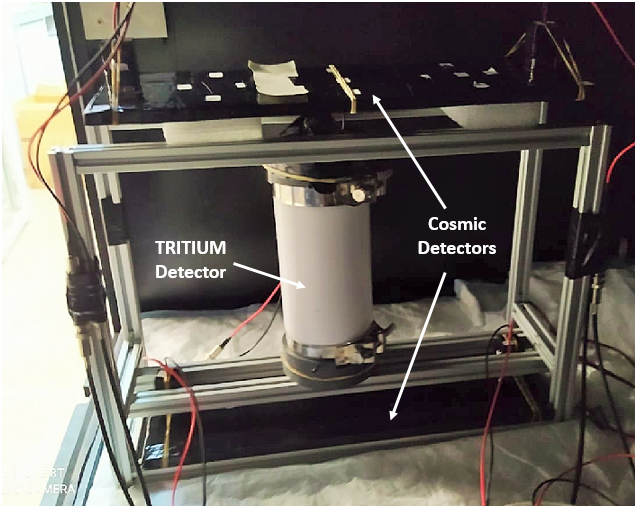
\includegraphics[scale=0.45]{3DesignPrinciples/34BackgroundRejectionSystem/Vetos_y_prototipo.png}
\caption{Cosmic veto and Tritium-IFIC 2 prototype in an aluminum mechanical structure developed by IFIC's mechanical engineering department.\label{fig:VetoAndPrototype}}
\end{figure}

%The cosmic veto is placed within the lead shielding so that, the weak radiation doesn't affect them with a false hard cosmic events detected.

A hard cosmic events simultaneous through both cosmic detectors is displayed in figure \ref{subfig:RealHardCosmicEvent}. Each cosmic detector has two photosensors. Hard cosmic events are rejected when both detectors are in coincidence with the electronic configuration given in Figure \ref{subfig:ElectronicConfiguraiton4PMT}. 

The TRITIUM detector is read out in anti-coincidence with the cosmic veto.  Random coincidence from cosmic two different hard cosmic events, one in each detector, shown in Figure \ref{subfig:FakeHardCosmicEvent} are negligible. The expected hard cosmic rate at sea level for muons, main contributor, is $70~\meter^{-2}\second^{-1}\steradian^{-1}$ \cite{PDG, HardCosmicMuonRate}, that is $7^{-3}~\cm^{-2}\second^{-1}\steradian^{-1}$, shown in the cosmic rate plot of Figure \ref{fig:HardCoscmicRate}. As time coincidences are triggered by logical gates of about $10~\nano\second$, the probability of recording two different hard cosmic events in temporal coincidence is less than $10^{-9}$ which is not worth considering.

\begin{figure}[h]
 \centering
  \subfloat[Real hard cosmic event.]{
   \label{subfig:RealHardCosmicEvent}
    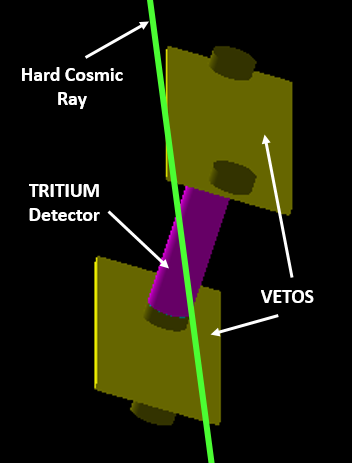
\includegraphics[width=0.45\textwidth]{3DesignPrinciples/34BackgroundRejectionSystem/Real_Event.png}}    
  \subfloat[Fake hard cosmic event.]{
   \label{subfig:FakeHardCosmicEvent}
    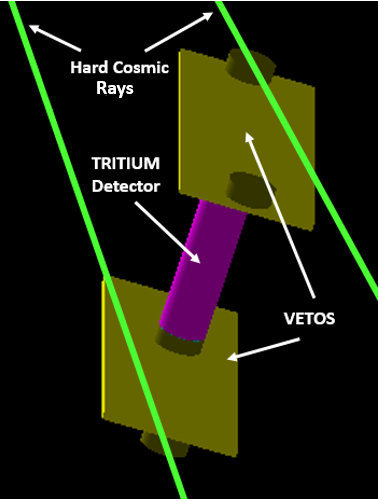
\includegraphics[width=0.45\textwidth]{3DesignPrinciples/34BackgroundRejectionSystem/Fake_Event.png}} 
   \caption{Hard cosmic events detected with the cosmic veto of TRITIUM: a) Affecting to the tritium measurement, b) Does not affecting to the tritium measurement.}
 \label{fig:HardCosmicEventsSimulation}
\end{figure}

\begin{figure}[h]
\centering
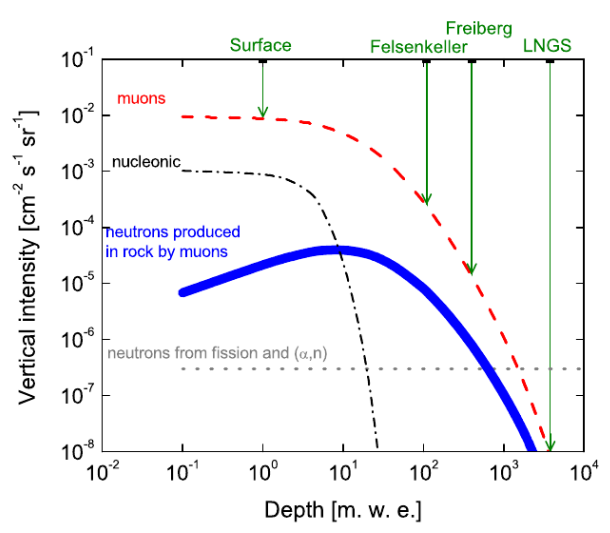
\includegraphics[scale=0.6]{3DesignPrinciples/34BackgroundRejectionSystem/HardCosmicRate.png}
\caption{Hard cosmic muon rate \cite{HardCosmicMuonRatePlot}.\label{fig:HardCoscmicRate}}
\end{figure}

The vetos are made of a plastic scintillator block from Epic-Crystal \cite{ScintillatorVeto}. Its properties are given in Table \ref{tab:ParametersScintillatorVeto} and its energy emission spectrum is displayed in Figure \ref{fig:EmissionEnergySpectrumVeto}.

\begin{table}[]
%%\centering
\begin{center}
\begin{tabular}{|c|c|c|}
%\hline
%Material & Refractive index \\
\hline \hline 
Base material & Polystyrene \\ \hline
Growth method & Polymeric \\ \hline
Density ($\gram/\cm^3$)& 1.05 \\ \hline
Refractive index & 1.58 \\ \hline
Soften temperature ($\degree$) & 75-80 \\ \hline
Light output (Anthracene) & 50-60\% \\ \hline
H/C raito & 1.1 \\ \hline
Emission peak (nm) & 415 (Blue) \\ \hline
Decay Time, (ns) & 2.4 \\ \hline
Hygroscopic & No \\ \hline
\end{tabular}
\caption{Properties of plastic scintillators from Epic-Crystals. \cite{ScintillatorVeto}}
\label{tab:ParametersScintillatorVeto}
\end{center}
\end{table}

\begin{figure}[]
\centering
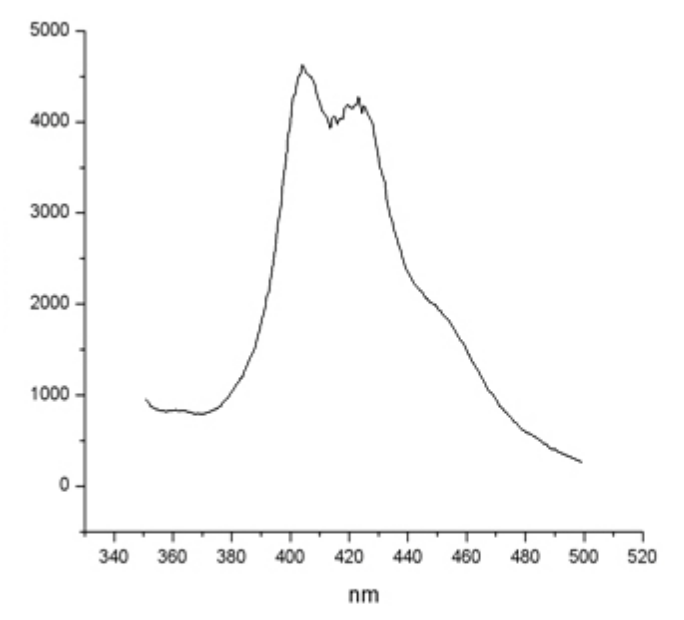
\includegraphics[scale=0.35]{3DesignPrinciples/34BackgroundRejectionSystem/EmissionEnergySpectrumVetos.png}
\caption{Emission energy spectrum of the plastic scintillation used for the cosmic vetos.\label{fig:EmissionEnergySpectrumVeto}~\cite{ScintillatorVeto}}
\end{figure}

The energy spectrum has a peak very close to that of the scintillating fibers used, so the same photosensors are used to read out them. The dimensions of the scintillator block are $45 \cdot{} 17 \dot{} 1~\cm^3$ and they are three foil wrapped by a layer of teflon, aluminum and black tape, exhibited in Figure \ref{fig:LayersVeto}. These layers prevent external photons from reaching the scintillator plastic and avoid photons generated by the scintillator plastic from escaping before reaching the photosensor. Two $2.5\cdot{} 2.5 ~\cm^2$ windows are made on the wrapping to allow reading by the photosensors.


\begin{figure}[h]
 \centering
  \subfloat[Scintillator without coating.]{
   \label{subfig:PlasticScintillatorNoCoating}
    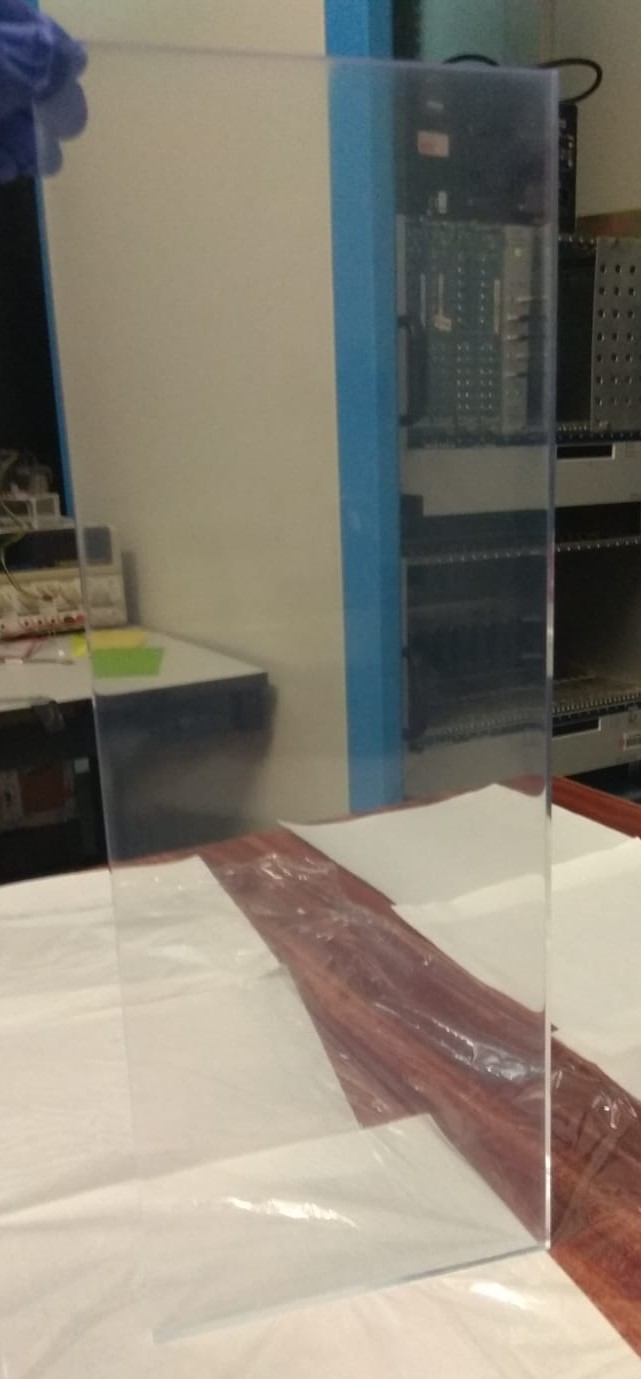
\includegraphics[width=0.23\textwidth]{3DesignPrinciples/34BackgroundRejectionSystem/NoCoating.jpeg}}    
  \subfloat[Teflon coating.]{
   \label{subfig:PlasticScintillatorTeflon}
    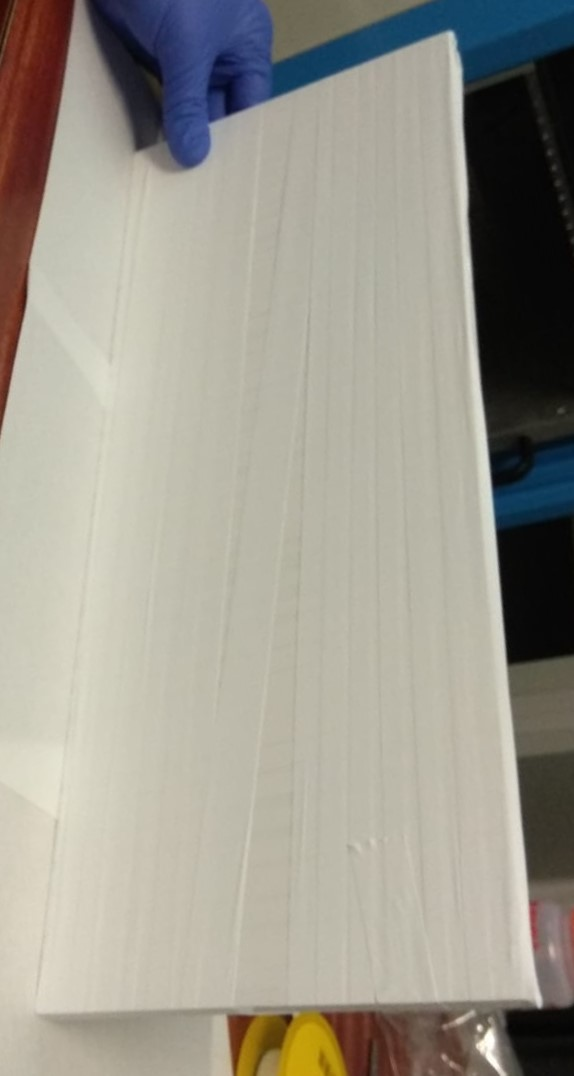
\includegraphics[width=0.23\textwidth]{3DesignPrinciples/34BackgroundRejectionSystem/TeflonCoating.jpeg}}  
  \subfloat[Aluminium coating.]{
   \label{subfig:PlasticScintillatorAluminium}
    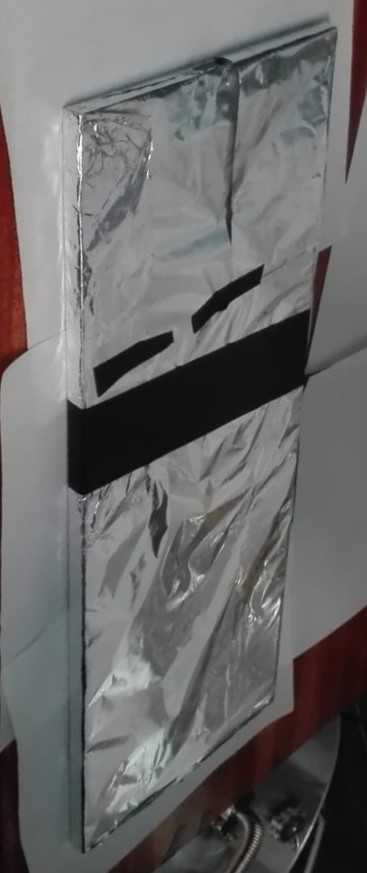
\includegraphics[width=0.23\textwidth]{3DesignPrinciples/34BackgroundRejectionSystem/AluminiumCoating.jpeg}}    
  \subfloat[Black tape coating.]{
   \label{subfig:PlasticScintillatorBlackTape}
    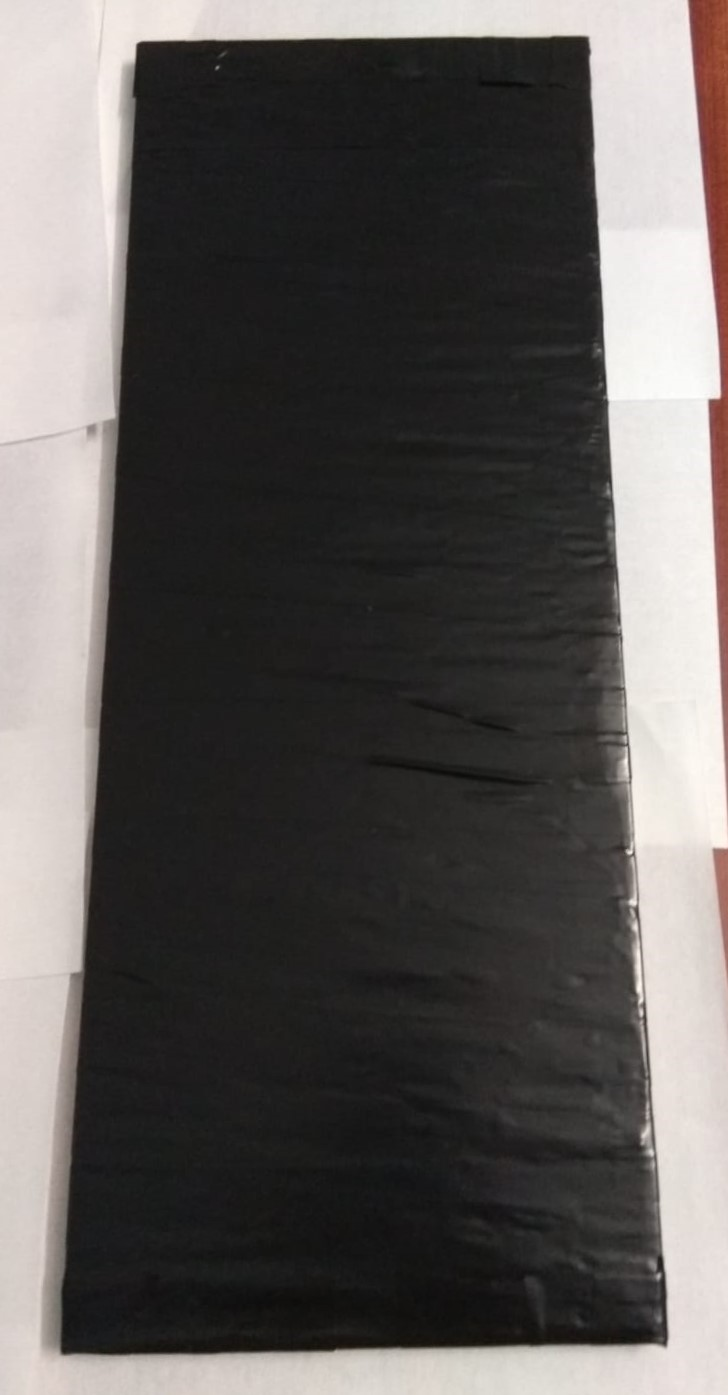
\includegraphics[width=0.23\textwidth]{3DesignPrinciples/34BackgroundRejectionSystem/BlackTapeCoating.jpeg}}
 \caption{Different layers used to cover of the cosmic veto.}
 \label{fig:LayersVeto}
\end{figure}

As previously mentioned, the expected hard cosmic rate at sea level is $7 \cdot{} 10^{-3}~\cm^{-2}\second^{-1}\steradian^{-1}$. As the solid angle of our detectors is $\omega=0.5434$, calculated by integrating the solid angle of one scintillator on the other, and the area of the veto is $765~\cm^2$, the expected hard cosmic rate on our cosmic vetos should be $2,909~$event$/\second$. Thus is important to determine the efficiency of the cosmic veto.